% !TEX program = pdflatex
% ============================================================
% GRETSI 2027 — Session historique — VERSION COURTE (24 planches)
% « Segmentation sémantique en télédétection »
% d'après M. Pastorino, G. Moser, J. Zerubia
% (../article/Martina_TSI_GRETSI_segmentation_semantique.pdf).
%
% Version resserrée de la présentation : 6 sections au lieu de 11,
% 20 planches d'exposé, pas de planches de section, pas de planche de
% crédits en back-up. Bibliographie réduite (54 entrées, revues et
% conférences abrégées) dans references.bib.
%
% Compilation : make  (latexmk + pdfLaTeX + biber, thème dans theme/)
% ============================================================
\documentclass[svgnames,9pt,aspectratio=169]{beamer}

\usepackage[french]{babel}
\usepackage{csquotes}
\usepackage{amsmath,amssymb,amsfonts,mathtools}
\usepackage{graphicx}
\usepackage{booktabs}
\usepackage{tikz}
\usetikzlibrary{positioning, shapes, arrows.meta, calc, fit, backgrounds, babel}

% ------------------------------------------------------------
% Le thème teste la primitive \draftmode. LuaTeX la fournit ; pdfTeX
% ne la connaît que depuis TeX Live 2024 (auparavant \pdfdraftmode).
% Cet alias permet de compiler avec les deux moteurs.
% ------------------------------------------------------------
\makeatletter
\ifdefined\draftmode\else
  \ifdefined\pdfdraftmode
    \let\draftmode\pdfdraftmode
  \else
    \providecommand{\draftmode}{0}%
  \fi
\fi
\makeatother

% ------------------------------------------------------------
% Thème Beamer Inria 2024 (dossier theme/, non modifié).
% ------------------------------------------------------------
\usetheme{inria}
\renewcommand{\thankyou}{Merci de votre attention.}

% ------------------------------------------------------------
% Bibliographie : ordre du fichier .bib = ordre de l'article.
% \nocite{*} est placé en tête de document pour que les numéros
% [n] des planches suivent cet ordre.
% ------------------------------------------------------------
\usepackage[backend=biber,style=numeric,sorting=none,
            maxbibnames=4,minbibnames=3,giveninits=true,
            doi=false,isbn=false,url=false,eprint=false]{biblatex}
\addbibresource{references.bib}
\renewcommand*{\bibfont}{\tiny}
\setlength{\bibitemsep}{0.35ex}

% ------------------------------------------------------------
% Logo Università di Genova (le thème Inria ne prévoit qu'un logo).
% Coordonnées textpos : fractions de \paperwidth / \paperheight.
% ------------------------------------------------------------
\newcommand{\logounige}[1][0.185]{%
  \begin{textblock}{#1}[1,0](0.955,0.085)
    
\includegraphics[width=\textwidth]{imgs/logos/logo_orizzontale_COLORE}
  \end{textblock}}

% ------------------------------------------------------------
% Commandes de mise en forme
% ------------------------------------------------------------
% Mise en évidence
\newcommand{\hl}[1]{\textcolor{inria-rouge}{\textbf{#1}}}

% Renvoi bibliographique en ligne : [n] en gris
\newcommand{\refc}[1]{\,\textcolor{gris_fonce_inria}{\footnotesize\cite{#1}}}

% Légende courte sous une figure (centrée)
\newcommand{\legende}[1]{%
  \par\vspace{0.4ex}{\scriptsize\color{gris_fonce_inria}\centering #1\par}}

% Crédit / copyright : dans le flux, juste sous les sous-légendes (centré)
\newcommand{\credit}[1]{%
  \par\vspace{0.35ex}{\tiny\color{gris_fonce_inria}\centering #1\par}}

% Références complètes citées sur la planche, tout en bas.
% Format compact : deux auteurs au plus, ni volume, ni numéro, ni pages.
\newtoggle{brefcite}
\AtEveryCitekey{\iftoggle{brefcite}%
  {\clearfield{pages}\clearfield{volume}\clearfield{number}}{}}
\newcommand{\bibline}[1]{%
  \par\hangindent=1.1em\hangafter=1\relax
  \mbox{\cite{#1}}~%
  \AtNextCite{\toggletrue{brefcite}%
    \defcounter{maxnames}{2}\defcounter{minnames}{1}}%
  \fullcite{#1}}
\newcommand{\biblio}[1]{%
  \begin{textblock}{0.92}[0,1](0.045,0.922)%
    \begingroup
    \fontsize{4.7}{5.2}\selectfont\raggedright\color{gris_fonce_inria}%
    \setlength{\parindent}{0pt}%
    \forcsvlist{\bibline}{#1}%
    \par                       % avant \endgroup : sinon la dernière ligne
    \endgroup                  % hérite de l'interligne du corps de planche
  \end{textblock}}

% Encadré de formule : liseré rouge Inria, fond gris très clair
\newcommand{\formulebox}[2][0.80]{%
  \begin{center}%
    \setlength{\fboxrule}{0.7pt}\setlength{\fboxsep}{7pt}%
    \fcolorbox{inria-rouge}{gris_fonce_inria!6}{%
      \begin{minipage}{#1\textwidth}\centering #2\end{minipage}}%
  \end{center}}

% Fil directeur de l'article : intégration progressive du contexte.
% Argument optionnel : numéro de l'étape à mettre en avant (0 = aucune).
\newcommand{\filrouge}[1][0]{%
  \begin{center}
  \begin{tikzpicture}[x=1mm,y=1mm,font=\scriptsize\bfseries]
    \foreach \i/\c/\t in {%
        0/inria-2024-bleu-azur/{Information\\spectrale locale},
        1/inria-2024-bleu-canard/{Cohérence\\spatiale},
        2/inria-2024-bleu-nuit/{Frontières,\\régions, objets},
        3/inria-2024-violet/{Apprentissage de\\représentations},
        4/inria-2024-rouge/{Modèles de\\fondation}}
      {%
        \node[fill=\c,text=white,align=center,text width=19mm,
              minimum height=11mm,inner sep=1.5pt] at ({\i*23},0) {\t};
        \ifnum\i>0
          \draw[-{Latex[length=1.8mm]},line width=0.8pt,gris_fonce_inria]
                ({\i*23-13},0) -- ({\i*23-10},0);
        \fi
      }
  \end{tikzpicture}
  \end{center}}

% Listes un peu aérées, sous-items légèrement décalés
% (le thème met \leftmarginii et \leftmarginiii à 0pt).
\setbeamertemplate{itemize/enumerate body begin}{\setlength{\itemsep}{0.85ex}}
\setbeamertemplate{itemize/enumerate subbody begin}{\setlength{\itemsep}{0.35ex}}
\setlength{\leftmarginii}{1.4em}
\setlength{\leftmarginiii}{1.4em}

% Sommaire
\addto\captionsfrench{\renewcommand{\contentsname}{Sommaire}}

% ------------------------------------------------------------
% Métadonnées
% ------------------------------------------------------------
% Neutralise la mise en forme des appels d'affiliation quand
% hyperref convertit \author en chaîne PDF.
\makeatletter
\pdfstringdefDisableCommands{%
  \let\textsc\@firstofone
  \let\emph\@firstofone
  \let\cite\@gobble
  \let\textsuperscript\@gobble
  \def\,{ }%
  \def\\{ }%
}
\makeatother

% NB : affiliations à confirmer avant diffusion.
\title{Segmentation sémantique en télédétection}
\subtitle{GRETSI 2027, session historique~\cite{pastorino2026segmentation}}
\date[GRETSI 2027]{2027}
\author{%
   Josiane \textsc{Zerubia}\\[2pt]
   \footnotesize Centre Inria d'Université Côte d'Azur, équipe \textsc{Ayana}\\[8pt]
   \footnotesize en collaboration avec Martina \textsc{Pastorino} et Gabriele \textsc{Moser}\\
   \footnotesize Università di Genova, \textsc{Diten}%
}
\institute{Sophia Antipolis}

\hypersetup{
   allcolors   = rouge_inria,
   pdfauthor   = {Josiane Zerubia, en collaboration avec Martina Pastorino et Gabriele Moser},
   pdftitle    = {Segmentation sémantique en télédétection},
   pdfsubject  = {GRETSI 2027 — session historique},
   pdfkeywords = {segmentation sémantique, télédétection, champs de Markov, CRF,
                  méthodes variationnelles, apprentissage profond, modèles de fondation}
}

% ============================================================
% ============================================================
\begin{document}
\nocite{*}   % fige la numérotation [n] sur l'ordre du fichier .bib

% ---- Page de titre -----------------------------------------
\frame{%
  \titlepage
  \logounige
  \biblio{pastorino2026segmentation}
}

% ---- Sommaire ----------------------------------------------
% Six sections : le sommaire tient sur une seule colonne.
\begin{frame}{Sommaire}
  % Dans une colonne, la boîte garde sa hauteur naturelle : les \vfill que
  % beamer insère entre les entrées ne s'étirent pas. Le \vspace* cale la
  % position verticale sur celle du PDF de référence.
  \vspace*{2.29pt}
  \begin{columns}[c,onlytextwidth]
    \begin{column}{\textwidth}
      \tableofcontents
    \end{column}
  \end{columns}
\end{frame}

% ============================================================
\section{Introduction}
% ============================================================
% Les sections ne sont pas introduites par une planche dédiée
% (contrairement à la version longue) : on enchaîne directement.

\begin{frame}{De l'image à la carte thématique}
  \begin{itemize}
    \item Associer à \hl{chaque pixel} une étiquette d'un ensemble prédéfini de classes
          sémantiques\refc{duda1973pattern}\refc{swain1978remote}\refc{richards1986remote} :
          problème étudié depuis des décennies sous les noms de \emph{classification
          supervisée}, \emph{pixel à pixel}, \emph{contextuelle}
    \item Produit une \hl{carte dense}, à distinguer de la segmentation qui partitionne
          en régions homogènes \emph{sans} leur associer de signification
    \item En télédétection : transformer les observations satellitaires en
          \hl{cartes d'occupation et d'utilisation du sol}
  \end{itemize}
  \vspace{0.4ex}
  \centerline{%
    \begin{minipage}[t]{0.22\textwidth}\centering
      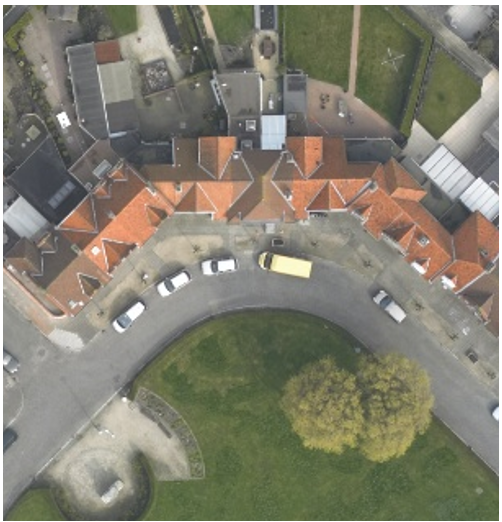
\includegraphics[height=2.0cm]{imgs/article/fig1a_zeebruges_image_aerienne}
      \legende{(a) image aérienne}
    \end{minipage}\hspace{3mm}%
    \begin{minipage}[t]{0.22\textwidth}\centering
      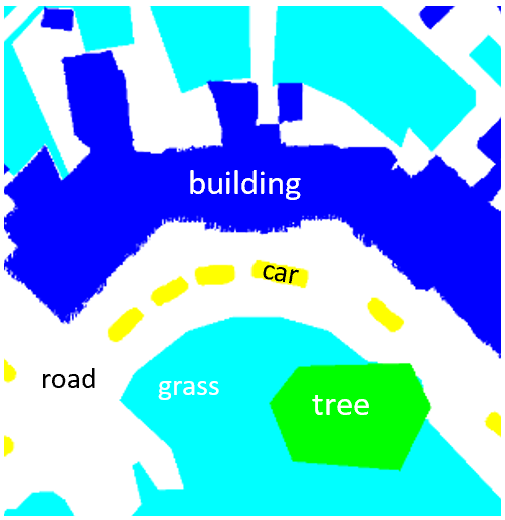
\includegraphics[height=2.0cm]{imgs/article/fig1b_zeebruges_carte_segmentation}
      \legende{(b) carte de segmentation}
    \end{minipage}}
  \credit{Jeu de données \emph{Zeebruges}, comité technique IADF de l'IEEE GRSS ;
    images et vérité terrain : Académie royale militaire belge et ONERA.}
  \biblio{duda1973pattern,swain1978remote,richards1986remote}
\end{frame}

\begin{frame}{Ce qui distingue la télédétection}
  \begin{itemize}
    \item \hl{Capteurs} hétérogènes : optique, radar à synthèse d'ouverture (RSO),
          LiDAR.
    \item \hl{Résolutions} spatiales et spectrales variables ; acquisitions
          \hl{multitemporelles} et \hl{multimodales}.
    \item \hl{Scènes géographiques complexes}, dont les propriétés varient selon les
          régions, les saisons et les conditions d'acquisition.
    \item Le domaine n'est donc pas une simple adaptation de la vision par ordinateur :
          il combine \hl{reconnaissance statistique}, \hl{traitement du signal},
          \hl{modélisation probabiliste} et \hl{apprentissage profond}.
  \end{itemize}
\end{frame}

\begin{frame}{Fil directeur}
  \formulebox{$I : \Omega \longrightarrow \mathbb{R}^{d}
              \qquad\text{puis}\qquad
              f : \Omega \longrightarrow \mathcal{C}$}
  \begin{itemize}
    \item $\Omega$ : domaine spatial ; $d$ : variables issues des bandes spectrales,
          polarisations RSO, mesures LiDAR, indices, MNT, etc.
    \item $\mathcal{C}$ : ensemble fini des classes sémantiques.
    \item L'histoire du domaine peut se lire comme une \hl{intégration progressive} de
          l'information spectrale, spatiale, contextuelle, puis multimodale.
  \end{itemize}
  \vspace{0.4ex}
  \filrouge
\end{frame}

% ============================================================
\section{Du pixel au contexte}
% ============================================================

\begin{frame}{Les premières approches : pixel à pixel}
  \begin{itemize}
    \item À la fin des années 1970 : Landsat (optique) et SeaSat (radar) créent le besoin
          de cartes d'occupation du sol
          automatiques\refc{schowengerdt2007remote}\refc{landgrebe2003signal}\refc{ulaby2015microwave}
    \item Chaque pixel est un vecteur d'observations
          $\mathbf{x} = (x_1,\dots,x_d)^{\mathsf{T}}$ : réponses radiométriques,
          intensités RSO, indices, données auxiliaires\refc{duda1973pattern}.
  \end{itemize}
  \formulebox{$\hat{\omega} \;=\; \arg\max_{\omega_i}\; P(\omega_i \mid \mathbf{x})$}
  \begin{itemize}
    \item Sous hypothèse gaussienne multivariée : \hl{classifieur MAP},
          « maximum a posteriori », référence pendant plusieurs
          décennies\refc{swain1978remote}\refc{richards1986remote}\refc{mather2004computer}
  \end{itemize}
  \biblio{duda1973pattern,swain1978remote,richards1986remote,schowengerdt2007remote,landgrebe2003signal,ulaby2015microwave,mather2004computer}
\end{frame}

\begin{frame}{Deux limites : dimension et indépendance}
  \begin{columns}[T,onlytextwidth]
    \begin{column}{0.50\textwidth}
      \begin{itemize}
        \item \hl{Malédiction de la dimension} (phénomène de
              Hughes)\refc{hughes1968mean} : plus de variables ne garantit pas de
              meilleures performances lorsque peu d'échantillons sont disponibles.
        \item \hl{Hypothèse d'indépendance des observations} : chaque pixel est décidé
              isolément, sans exploiter son voisinage or les objets géographiques sont
              fortement corrélés spatialement : parcelle agricole, forêt, zone urbaine,
              réseau routier
        \item Conséquence : \hl{cartes bruitées}, d'autant plus que la résolution
              spatiale augmente
      \end{itemize}
    \end{column}
    \begin{column}{0.48\textwidth}\centering
      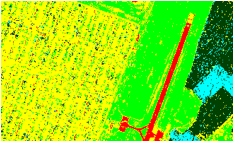
\includegraphics[width=0.72\textwidth]{imgs/article/fig2b_classification_pixel_a_pixel}
      \legende{Classification pixel à pixel : effet « poivre et sel »\refc{moser2013landcover}}
    \end{column}
  \end{columns}
  \biblio{hughes1968mean,moser2013landcover}
\end{frame}

\begin{frame}{Méthodes discriminantes et d'ensemble}
  \begin{itemize}
    \item À partir de la fin des années 1990 : estimer \hl{directement les frontières
          de décision}, plutôt que la loi des observations.
    \item \hl{SVM} : maximisation de la marge ; bonne généralisation en grande
          dimension\refc{vapnik1998statistical}\refc{cortes1995support}\refc{campsvalls2009kernel}\refc{mountrakis2011support}.
    \item \hl{Noyaux} : non-linéarité sans perdre la convexité ; nombreux développements
          pour les observations géospatiales\refc{scholkopf2002learning}.
    \item \hl{Forêts aléatoires} : vote d'arbres de décision appris sur des sous-ensembles
          aléatoires ; robustesse, peu de réglages, importance des
          variables\refc{breiman2001random}\refc{gislason2006random}.
    \item Mais ces méthodes restent des classifieurs \hl{essentiellement pixel à pixel}
          lorsqu'elles sont appliquées aux observations locales.
  \end{itemize}
  \biblio{vapnik1998statistical,cortes1995support,scholkopf2002learning,campsvalls2009kernel,mountrakis2011support,breiman2001random,gislason2006random}
\end{frame}

\begin{frame}{L'apport du contexte spatial}
  \begin{columns}[T,onlytextwidth]
    \begin{column}{0.32\textwidth}\centering
      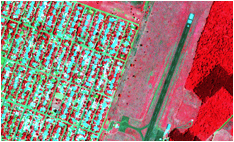
\includegraphics[width=0.84\textwidth]{imgs/article/fig2a_ikonos_fausses_couleurs}
      \legende{(a) image IKONOS}
    \end{column}
    \begin{column}{0.32\textwidth}\centering
      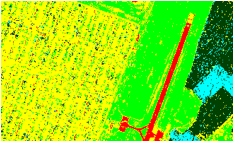
\includegraphics[width=0.84\textwidth]{imgs/article/fig2b_classification_pixel_a_pixel}
      \legende{(b) pixel à pixel}
    \end{column}
    \begin{column}{0.32\textwidth}\centering
      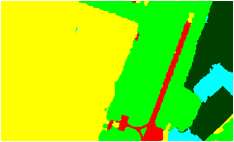
\includegraphics[width=0.84\textwidth]{imgs/article/fig2c_classification_contextuelle}
      \legende{(c) contextuelle}
    \end{column}
  \end{columns}
  \credit{Image IKONOS, 4~m, 3 bandes, fausses couleurs ; cartes de
    segmentation \cite{moser2013landcover}.}
  \begin{itemize}
    \item En télédétection, les objets géographiques présentent une \hl{forte cohérence
          spatiale} : parcelles, forêts, zones urbaines, réseaux routiers.
    \item Les étiquettes doivent être estimées \hl{conjointement}, pas pixel par pixel.
  \end{itemize}
  % ATTENTION — défaut connu, reproduit tel quel : `haralick1985image` n'est PAS
  % dans references.bib (la bibliographie courte ne la reprend pas), si bien que
  % le bandeau du bas affiche « [haralick1985image] haralick1985image » au lieu
  % d'une référence. C'est ce qu'imprime le PDF de reference/, d'où le maintien
  % à l'identique. Pour corriger : soit retirer la clé de la ligne ci-dessous
  % (la planche ne la cite nulle part ailleurs), soit réintroduire l'entrée dans
  % references.bib — mais cela décalerait tous les numéros [n] suivants.
  \biblio{richards1986remote,haralick1985image,solberg1996markov,moser2013landcover}
\end{frame}

% ============================================================
\section{Modèles markoviens et bayésiens}
% ============================================================

\begin{frame}{Les champs de Markov : première formalisation}
  \begin{itemize}
    \item Les étiquettes deviennent des variables aléatoires définies sur un \hl{graphe
          de voisinage}\refc{geman1984stochastic}\refc{besag1986statistical}\refc{kato2012markov}.
    \item Sous les hypothèses de Markov et l'équivalence avec les distributions de Gibbs,
          l'estimation MAP devient une \hl{minimisation d'énergie}.
  \end{itemize}
  \formulebox{$\hat{Y} \;=\; \arg\max_{Y} P(Y \mid X)
              \qquad\Longleftrightarrow\qquad
              \hat{Y} \;=\; \arg\min_{Y} U(Y \mid X)$}
  \begin{itemize}
    \item $X$ : observations ; $Y$ : carte d'étiquettes à estimer.
    \item Les MRF fournissent un cadre général pour relier données locales et cohérence
          spatiale.
  \end{itemize}
  \biblio{geman1984stochastic,besag1986statistical,kato2012markov}
\end{frame}

\begin{frame}{Attache aux données + régularisation}
  \formulebox{$U(Y \mid X) \;=\; U_d(Y \mid X) \;+\; \beta\, U_r(Y \mid X)$}
  \begin{columns}[T,onlytextwidth]
    \begin{column}{0.56\textwidth}
      \begin{itemize}
        \item $U_d$ : \hl{attache aux données}, dérivée de la vraisemblance.
        \item $U_r$ : \hl{régularisation spatiale}, favorise la cohérence entre pixels
              voisins.
        \item $\beta$ : compromis fidélité / régularité.
        \item Voisinages du 1\textsuperscript{er} ou du 2\textsuperscript{d} ordre ;
              les potentiels de clique \hl{pénalisent les changements} de classe entre
              \hl{pixels adjacents}\refc{kato2012markov}
      \end{itemize}
    \end{column}
    \begin{column}{0.42\textwidth}\centering
      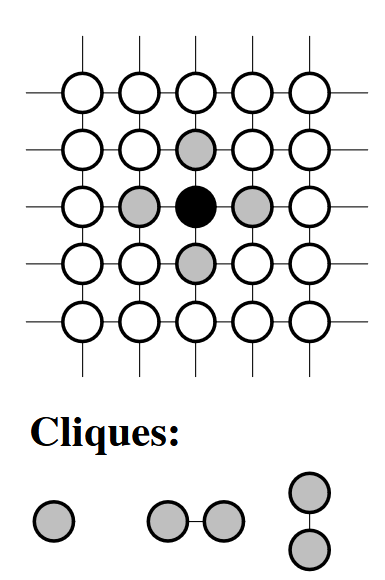
\includegraphics[height=2.5cm]{imgs/article/fig3a_voisinage_ordre1_cliques}%
      \hspace{2mm}%
      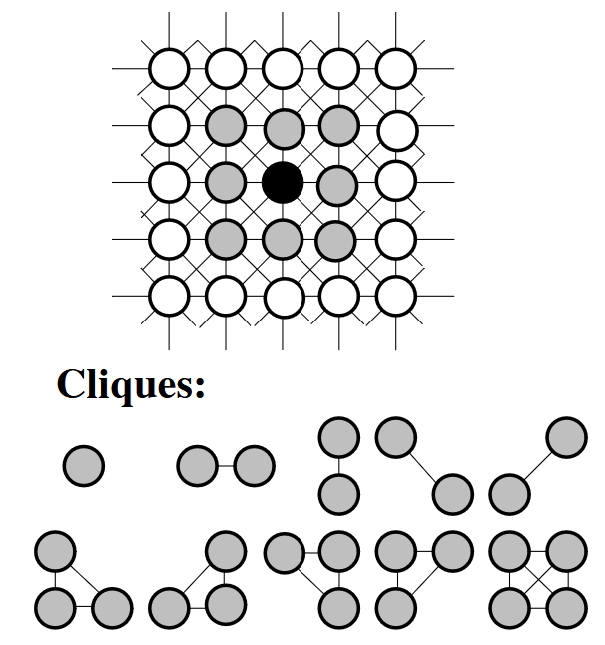
\includegraphics[height=2.5cm]{imgs/article/fig3b_voisinage_ordre2_cliques}
      \legende{(a) 1\textsuperscript{er} ordre \quad (b) 2\textsuperscript{d} ordre}
      \credit{Voisinages entre pixels dans une grille et cliques
        associées \cite{kato2012markov}.}
    \end{column}
  \end{columns}
  \biblio{kato2012markov}
\end{frame}

\begin{frame}{Optimisation et usages des MRF}
  \begin{itemize}
    \item Trouver la configuration optimale est un problème d'optimisation combinatoire
          difficile.
    \item Stratégies : \hl{ICM}, \hl{recuit simulé}\refc{kirkpatrick1984optimization},
          échantillonneur de \hl{Gibbs}\refc{geman1984stochastic},
          \hl{coupes de graphes}\refc{boykov2001fast}, propagation de croyance avec
          boucles\refc{tanaka2003loopy}.
    \item Applications : classification contextuelle, segmentation multisource,
          restauration, détection de changements, fusion optique / radar /
          LiDAR\refc{solberg1996markov}\refc{derin1987modeling}\refc{moser2013combining}.
    \item Au-delà des applications : une \hl{formulation probabiliste générale} de la
          régularisation spatiale.
  \end{itemize}
  \biblio{geman1984stochastic,solberg1996markov,kirkpatrick1984optimization,boykov2001fast,tanaka2003loopy,derin1987modeling,moser2013combining}
\end{frame}

\begin{frame}{Des MRF aux CRF : un pont vers le profond}
  \begin{itemize}
    \item Les champs conditionnels aléatoires représentent directement $P(Y \mid X)$
          plutôt que la loi jointe\refc{lafferty2001conditional} : ils facilitent l'usage
          de \hl{caractéristiques discriminantes complexes}.
    \item \hl{CRF entièrement connectés} : contours des objets mieux
          préservés\refc{krahenbuhl2011efficient}.
    \item Intégration aux réseaux profonds : modules de raffinement, \hl{couches
          différentiables}\refc{zheng2015conditional} ; cadres markoviens hiérarchiques
          et CRF appris\refc{pastorino2021multisensor}\refc{pastorino2022semantic}\refc{pastorino2024crfnet}\refc{voisin2013classification}.
    \item \hl{L'idée qui traverse le domaine} : une carte doit être compatible avec les
          observations locales \emph{et} avec l'organisation spatiale de la scène.
  \end{itemize}
  \biblio{lafferty2001conditional,krahenbuhl2011efficient,zheng2015conditional,pastorino2021multisensor,pastorino2022semantic,pastorino2024crfnet,voisin2013classification}
\end{frame}

% ============================================================
\section{Représentations spectro-spatiales et variationnelles}
% ============================================================

\begin{frame}{Enrichir la représentation, pas seulement les étiquettes}
  \begin{itemize}
    \item Les modèles contextuels régularisent les \hl{étiquettes} ; les méthodes
          spectro-spatiales enrichissent les \hl{descripteurs} avant la
          classification\refc{landgrebe2003signal}
    \item Avec l'augmentation des résolutions, les signatures radiométriques seules
          deviennent insuffisantes.
    \item Texture, forme, taille, organisation spatiale et relations de voisinage
          deviennent \hl{aussi discriminantes que les valeurs
          spectrales}\refc{dellepiane1991sar}.
    \item Cette logique prépare les représentations multi-échelles apprises par les
          réseaux profonds\refc{blaschke2010object}.
  \end{itemize}
  \biblio{landgrebe2003signal,blaschke2010object,dellepiane1991sar}
\end{frame}

\begin{frame}{Morphologie mathématique et profils multi-échelles}
  \begin{columns}[T,onlytextwidth]
    \begin{column}{0.32\textwidth}\centering
      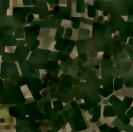
\includegraphics[height=2.15cm]{imgs/article/fig4a_erosion}
      \legende{érosion}
    \end{column}
    \begin{column}{0.32\textwidth}\centering
      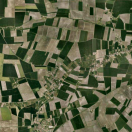
\includegraphics[height=2.15cm]{imgs/article/fig4b_image_originale_rvb}
      \legende{image originale RVB}
    \end{column}
    \begin{column}{0.32\textwidth}\centering
      
\includegraphics[height=2.15cm]{imgs/article/fig4c_dilatation}
      \legende{dilatation}
    \end{column}
  \end{columns}
  \credit{Érosion et dilatation de l'image satellite originale RVB.}
  \begin{itemize}
    \item Opérateurs : érosion, dilatation, ouvertures,
          fermetures\refc{serra1982image}\refc{soille2003morphological}.
    \item \hl{Profils morphologiques étendus} et \hl{profils d'attributs} décrivent
          forme, taille et contraste à plusieurs
          échelles\refc{benediktsson2005classification}\refc{dallamura2010morphological}\refc{fauvel2008spectral}.
  \end{itemize}
  \biblio{serra1982image,soille2003morphological,benediktsson2005classification,dallamura2010morphological,fauvel2008spectral}
\end{frame}

\begin{frame}{Méthodes variationnelles : régulariser la solution}
  \begin{itemize}
    \item Démarche complémentaire : intégrer directement la cohérence spatiale dans la
          formulation du problème.
    \item La segmentation est formulée comme une \hl{minimisation d'énergie} combinant
          fidélité aux observations et régularité spatiale ou
          géométrique \refc{samson2000variational}.
  \end{itemize}
  \formulebox{$E(u) = \text{fidélité aux données} +
              \lambda\,\text{régularité spatiale/géométrique}$}
  \begin{itemize}
    \item La fonctionnelle de \hl{Mumford--Shah} est l'un des modèles
          fondateurs\refc{mumford1989optimal}.
    \item Les principes de compromis données/régularité, multi-échelle et fusion seront
          repris sous des formes apprises dans l'apprentissage profond.
  \end{itemize}
  \biblio{mumford1989optimal,samson2000variational}
\end{frame}

% ============================================================
\section{Apprentissage profond et modèles de fondation}
% ============================================================

\begin{frame}{Apprendre profond}
  \vspace*{2.06pt}% calage vertical sur le PDF de référence
  \begin{columns}[T,onlytextwidth]
    \begin{column}{0.52\textwidth}
      \begin{itemize}
        \item 2012 la bascule : \hl{AlexNet} démontre une amélioration spectaculaire en
              classification d'images naturelles\refc{krizhevsky2012imagenet}
        \item Changement : apprendre conjointement les représentations et la fonction de
              décision directement à partir des données.
        \item \hl{FCN} : prédiction dense à l'échelle du pixel.
      \end{itemize}
    \end{column}
    \begin{column}{0.43\textwidth}\centering
      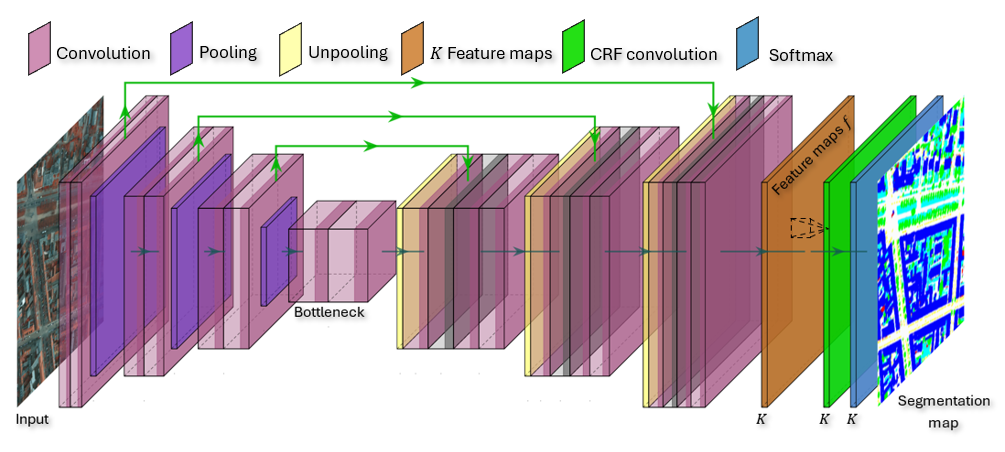
\includegraphics[width=0.95\textwidth]{imgs/article/fig6_fcn_potsdam}
      \legende{Architecture FCN appliquée à Potsdam}
    \end{column}
  \end{columns}
  \vspace{1.2ex}
  \begin{itemize}
    \item \hl{U-Net} : connexions de saut pour restituer l'information spatiale.
    \item \hl{DeepLab} : convolutions dilatées et représentations multi-échelles pour
          élargir le champ réceptif.
  \end{itemize}
  \biblio{krizhevsky2012imagenet,long2015fully,ronneberger2015unet,chen2018encoder,audebert2018beyond,ma2019deep}
\end{frame}

\begin{frame}{Transformers, auto-supervisé et modèles de fondation}
  % Colonnes hors `onlytextwidth` : le bloc déborde légèrement des marges de texte,
  % ce qui laisse la place à la figure 7 (la plus large de la présentation).
  \vspace*{-1.24pt}% calage vertical sur le PDF de référence
  \begin{columns}[T]
    \begin{column}{0.58\textwidth}
      \begin{itemize}
        \item Les CNN restent limités par le besoin en annotations et par la
              modélisation des dépendances à longue portée.
        \item Les mécanismes d'\hl{attention} et les transformers représentent mieux les
              interactions entre régions
              distantes\refc{vaswani2017attention}\refc{dosovitskiy2021image}.
        \item L'\hl{auto-supervision} exploite de grands volumes d'images satellitaires
              non annotées pour apprendre des représentations
              transférables\refc{he2022masked}.
      \end{itemize}
    \end{column}
    % Figure calée sur le PDF de référence : bord gauche à ras de la colonne
    % (pas de \centering ici — \legende se centre toute seule) et largeur
    % 1,0038 fois la colonne, soit 154,9 pt.
    \begin{column}{0.41\textwidth}
      \vspace{1.65ex}
      \noindent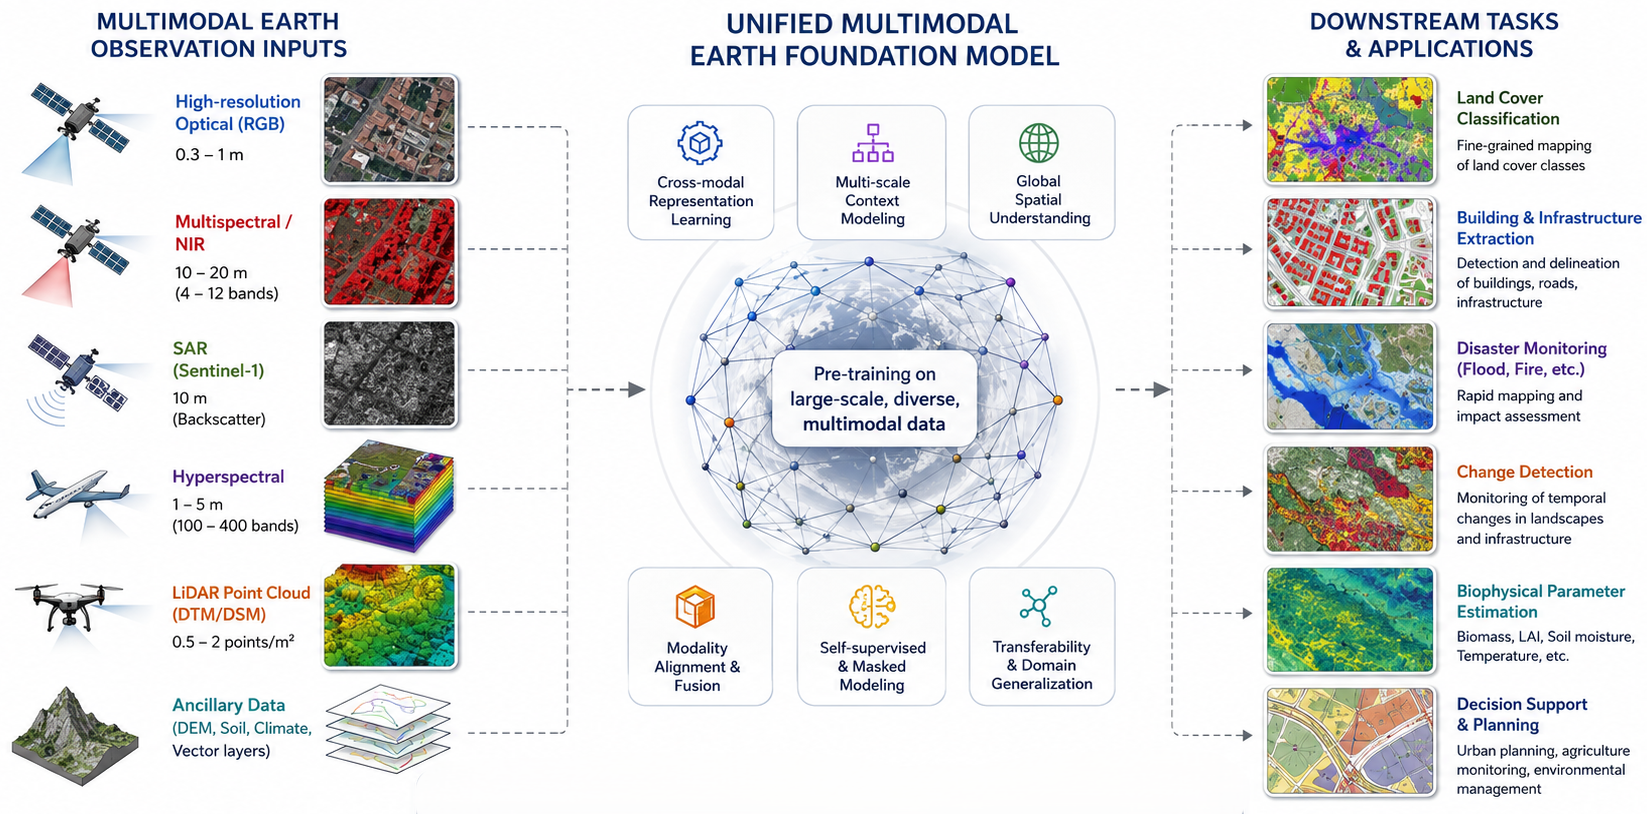
\includegraphics[width=1.0038\textwidth]{imgs/article/fig7_modele_fondation_geospatial}
      \legende{Principe d'un modèle de fondation géospatial}
    \end{column}
  \end{columns}
  \begin{itemize}
    \item Objectif : passer d'un modèle spécialisé à des représentations \hl{générales,
          multimodales et transférables (modèles de fondation
          geospatiaux)}\refc{xiao2025foundation}.
  \end{itemize}
  \biblio{vaswani2017attention,dosovitskiy2021image,he2022masked,xiao2025foundation}
\end{frame}

% ============================================================
\section{Défis ouverts}
% ============================================================

\begin{frame}{Défis ouverts}
  \begin{itemize}
    \item \hl{Généralisation} entre régions, saisons, capteurs et résolutions.
    \item \hl{Manque d'annotations} : coût élevé des vérités terrain, déséquilibre entre
          classes, labels imparfaits.
    \item \hl{Fusion multimodale} : optique, RSO, LiDAR, séries temporelles et données
          auxiliaires.
    \item \hl{Robustesse} : changements de distribution, nuages, bruit, artefacts,
          événements rares.
    \item \hl{Interprétabilité} : comprendre et contrôler les décisions de modèles de
          plus en plus grands.
  \end{itemize}
\end{frame}

\begin{frame}{Conclusion : une histoire non linéaire}
  \begin{itemize}
    \item Pas une trajectoire allant simplement des classifieurs statistiques aux
          réseaux profonds, mais la \hl{convergence de plusieurs familles de méthodes} :
          classification statistique, méthodes à noyaux, méthodes d'ensemble, modèles
          contextuels, champs de Markov, méthodes variationnelles, géométrie
          stochastique, apprentissage profond, modèles de fondation
    \item Une lecture unifiée : l'\hl{intégration progressive de niveaux croissants de
          contexte}
  \end{itemize}
  \vspace{0.6ex}
  \filrouge
  \vspace{0.4ex}
  \begin{itemize}
    \item Un principe récurrent : \hl{attache aux données $+$ régularisation}, des
          champs de Markov aux fonctions de perte des réseaux profonds
  \end{itemize}
\end{frame}

% ---- Merci -------------------------------------------------
\frame{\merci}

% ============================================================
% Annexe : bibliographie complète
% ============================================================
\begin{frame}[allowframebreaks]{Références}
  \printbibliography[heading=none]
\end{frame}

\end{document}
